\chapter{Systems and Implementations}
\label{chpt:sytems}

\section{Aurox Clarity System}
\label{sec:aurox}

Confocal laser scanning microscopy (CLSM) is, traditionally, a
point-scanning microscopy technique pioneered with the objective of
discarding the scattered illumination light and the out-of-focus
excited fluorescence when imaging biological
samples\cite{minsky1988memoir}. Discarding the out-of-focus light
yields images with high contrast and good optical
sectioning\cite{nwaneshiudu2012introduction}. The original Minsky
design struggled with a low-frame rate. Advances in technology have
led to improved scanning speeds and therefore improved image frame
rates which, for modern CLSM set-ups, is generally on the order of 
milliseconds per 2D frame\cite{schermelleh2010guide,xiao1988real}. For many 
dynamic biological processes this is still insufficient, which lead to the 
development of (among other things) the Nipkow-Petran spinning disk setup 
which allows for video rate confocal 
imaging\cite{egger1967new,fuseler2018types,tsien1995video}. Hence, spinning 
disk confocal microscopes are frequently used for imaging live biological 
processes.

The Nipkow-Petran design does have disadvantage in that it discards 
$\sim99\%$ of both excitation and emission light in order to achieve good 
optical sectioning and \textit{xy}-resolution\cite{kino1995intermediate}. 
This can lead to poor signal-to-noise ratio (SNR) in fluorescence imaging if 
sufficiently strong fluorophores aren't used\cite{semwogerere2005confocal}. 
This disadvantage is somewhat mitigated - but not entirely overcome - in 
systems employing microlens arrays such as the Yokogawa 
systems\cite{wang2005performance}. Another design exists called a Correlation 
Disk which uses light emitting diodes (LEDs) as the illumination light source 
in conjunction with a patterned disk which is placed in a location shared by 
both the excitation and emission beam 
paths\cite{juskaitis1996efficient,wilson1996confocal,neil1997method}. The 
Aurox Clarity module employs just such an approach to achieve real-time 
confocal imaging with a significantly increased light budget (only $50\%-75\%$ of the emitted light is discarded compared the typical $\sim99\%$). This approach relies on good correlation between the 
grid patterns present in both the excitation and emission paths, which is 
degraded by optical aberrations\cite{hussain2020wavefront}. Therefore, the 
Aurox Clarity System incorporates both the Aurox Clarity module for fast, 
laser-free confocal imaging and a deformable mirror (DM) for aberration 
correction.

\subsection{Aurox Clarity System Optical Set-up}
\label{subsec:aurox_optics}

Figure~\ref{fig:aurox_beam_path} shows the complete optical schematic of the Aurox Clarity system. Its base is an iX71 Olympus microscope body with a AMEP4694 $60\times$, 1.42 NA oil objective and P-736.ZR1S PI-nano Z Microscope Scanner piezo Z-stage. Ordinarily, the Clarity module would be attached to the side port of the microscope body. The Mirao52e, a 52-actuator DM, must be placed in a plane conjugate to the back pupil plane in order to correct for the aberrations. To achieve this, the Clarity module was separated from the main microscopy body by a 4f, unity magnification telescope. The 4f telescope re-images the image plane close to the side port onto input port of the Clarity module and the DM was placed at the intermediate pupil plane. The Mirao52e DM was calibrated using a separate set-up not shown which uses a technique based on deflectometry\cite{trumper2016instantaneous,huang2017close}. A Photometrics PrimeBSI camera was attached to the Camera port of the Aurox Clarity module. A pE-300 Ultra CoolLED was attached to the Illumination light input port.

\begin{figure}[h]
	\begin{subfigure}{0.48\textwidth}
		\centering
		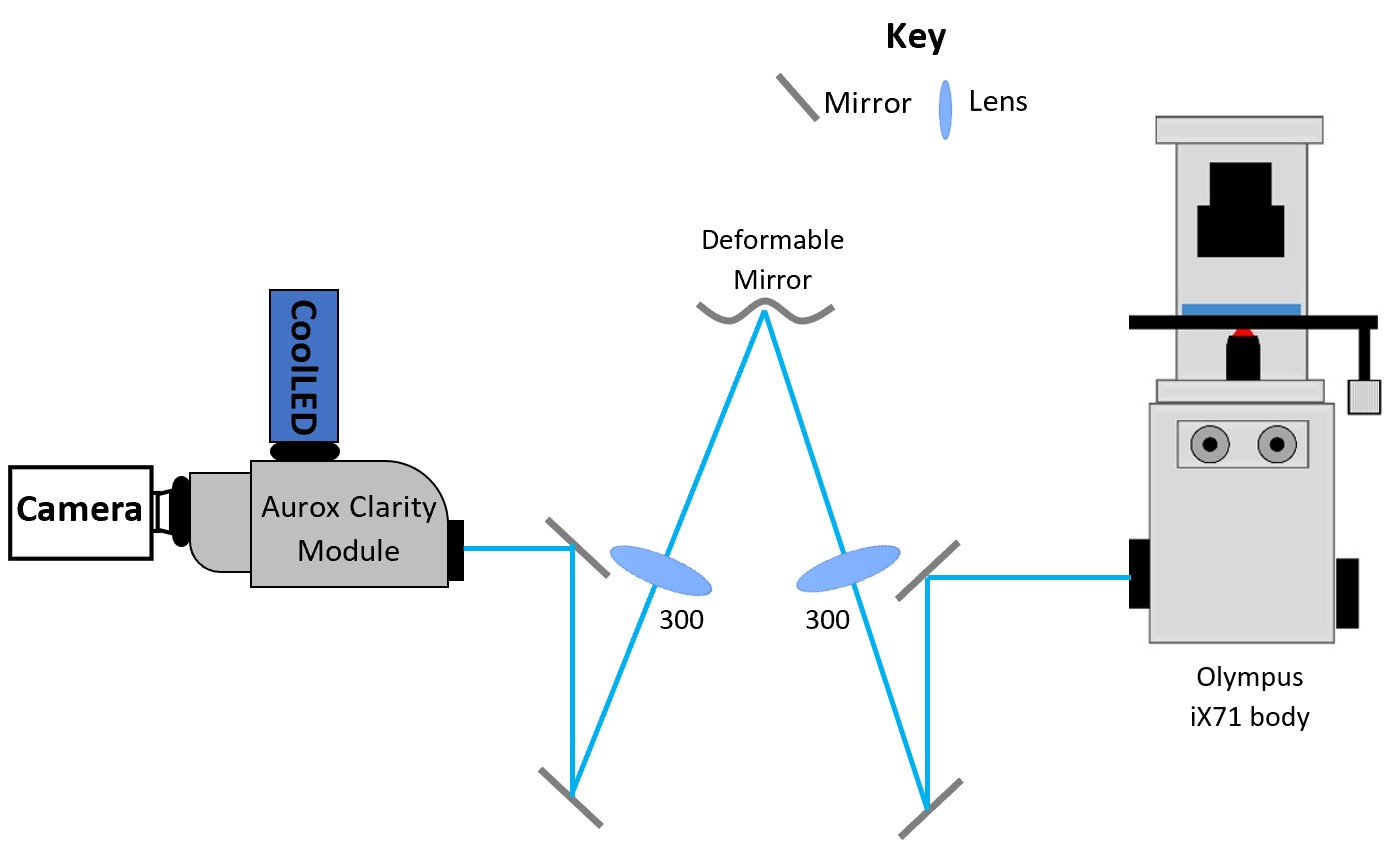
\includegraphics[width=\linewidth]{images/Aurox_beam_path.jpg}
		\caption{}
		\label{fig:aurox_beam_path}
	\end{subfigure}
	\begin{subfigure}{0.48\textwidth}
		\centering
		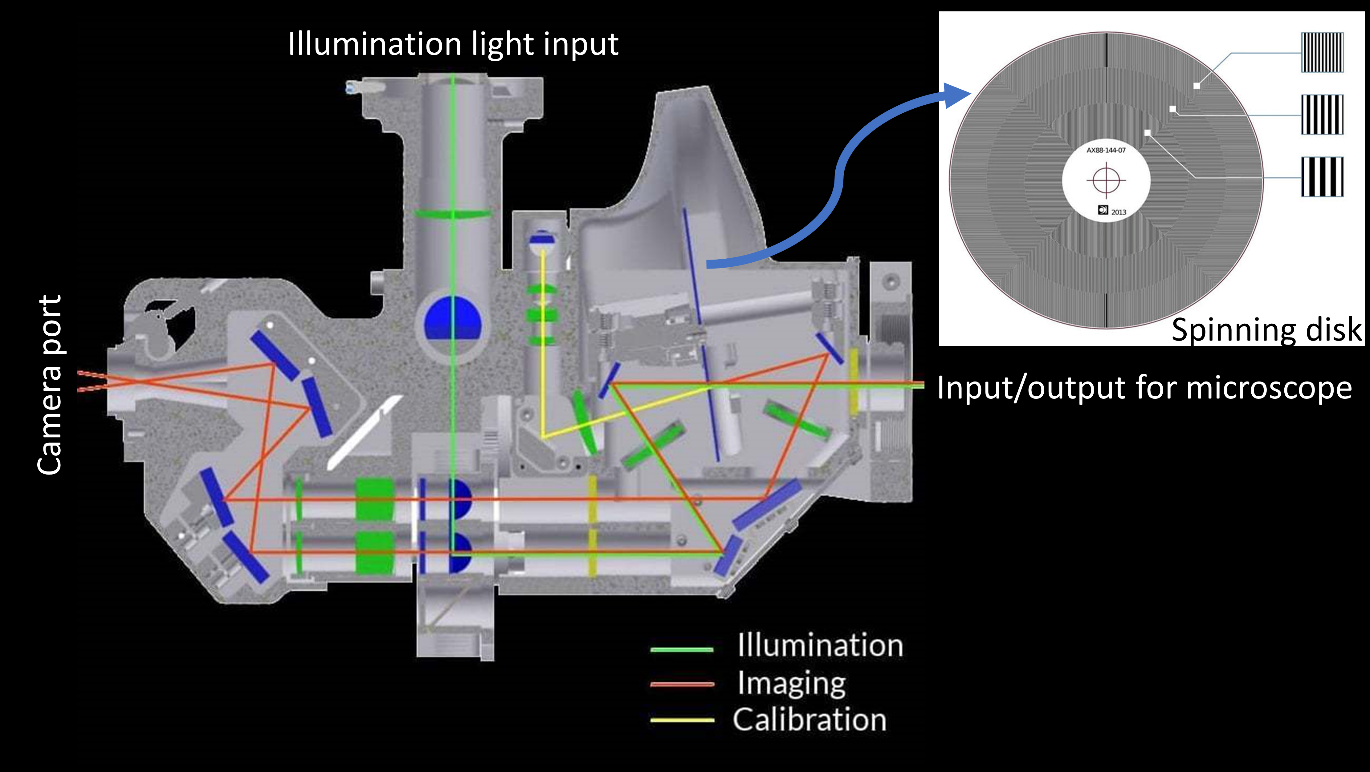
\includegraphics[width=\linewidth]{images/aurox_clarity_internal.png}
		\caption{}
		\label{fig:aurox_clarity_internal}
	\end{subfigure}
	\caption[Aurox system beam path layout]{Aurox system beam path layout \textbf{(a)} The complete imaging beam path for the Aurox Clarity System. The excitation and emission beam paths are identical up to the Aurox Clarity module \textbf{(b)} The internal beam paths for the Aurox Clarity module (Modified with permission from Aurox Ltd., Copyright Aurox Ltd.)}
	\label{fig:aurox_system}
\end{figure}

The excitation and emission beam paths are identical from the input/output microscope port to the focal plane of the objective. The differing beam paths for the excitation and emission light within the Clarity module are shown in Figure~\ref{fig:aurox_clarity_internal}. The excitation light impinges on the spinning disk and is either transmitted by the disk or discarded. The emission light impinges on the spinning disk in the opposite direction. The emission light from the focal plane of the objective is transmitted by the disk and is directed to one half of the PrimeBSI camera chip. The rest of the emission light is reflected off the disk and directed to the opposite half of the PrimeBSI camera chip. The Calibration light source generated within the Clarity module is used to align the two halves of the PrimeBSI camera chip to one another. A set of dichroic filter cubes are used to select both the excitation and emission wavelengths. There are four available dichroic filter cubes which can be selected:

\begin{enumerate}
	\item Dichroic filter 1: Excitation 466nm/FWHM 40nm, Emission 525nm /FWHM 45nm
	\item Dichroic filter 2: Excitation 554nm /FWHM 23nm, Emission 609nm /FWHM 54nm
	\item Dichroic filter 3: Excitation 578nm /FWHM 21nm, Emission 641nm /FWHM 75nm
	\item Dichroic filter 4: Excitation 392nm /FWHM 23nm, Emission 447nm /FWHM 60nm  
\end{enumerate}

The Aurox Clarity system was built by Dr Syed Hussain and Mr Toshiki Kubo. The innovation which this thesis presents is the successful implementation of Microscope-AOtools to provide control of the deformable mirror and therefore system and sample aberration correction which enabled high-quality imaging at depth.

\subsection{Image Formation in Aurox Clarity Module}
\label{sec:Aurox_image_formation}

Figure~\ref{fig:confocal_schematic} shows a simplified schematic 
for a Nipkow-Petran spinning disk confocal microscope. The 
excitation illumination passes through an aperture mask, which is 
then imaged onto the sample. This aperture mask consists of a 
number of pinholes packed closely together, illuminating a number 
of focal spots at once. The excitation light then passes back 
through the aperture mask where the out-of-focus light is 
discarded by the pinhole array\cite{egger1967new,fuseler2018types}.

\begin{figure}[h]
	\centering
	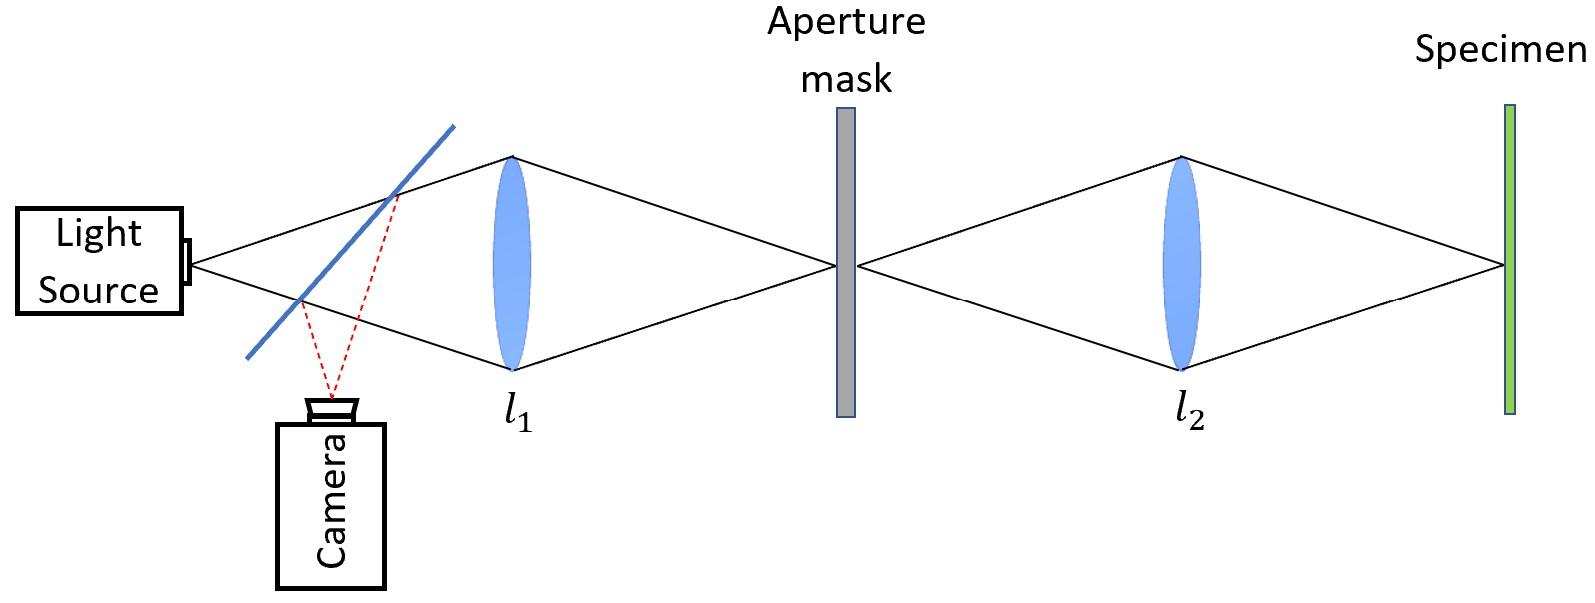
\includegraphics[width=\textwidth]{images/confocal_schematic.jpg}
	\caption[Simplified Nipkow-Petran confocal layout]{A schematic diagram showing a simplified layout for a Nipkow-Petran spinning disk confocal microscope}
	\label{fig:confocal_schematic}
\end{figure}

Consider a transmissive optical system as shown in 
Figure~\ref{fig:optical_system_schematic}. For an incoherent 
light source, immediately after the detector mask the 
intensity, $I\left(\textbf{x}_{2}\right)$, is given by:

\begin{equation}\label{eq:intensity_after_detector}
I\left(\textbf{x}_{2}\right) = \int S\left(\textbf{x}_{1}\right) D\left(\textbf{x}_{2}\right) \left| \int h_{1}\left(\textbf{x}_{0} + \frac{\textbf{x}_{1}}{M}\right) \tau\left(\textbf{x}_{0}\right) h_{2}\left(\textbf{x}_{0} + \frac{\textbf{x}_{2}}{M}\right)d\textbf{x}_{0}\right|^{2}d\textbf{x}_{1},
\end{equation}

where $S\left(\textbf{x}_{1}\right)$ is the intensity 
sensitivity of the source mask, $D\left(\textbf{x}_{2}\right)$ 
is the detector mask, $\tau\left(\textbf{x}_{0}\right)$ is 
the amplitude transmittance function of the aperture mask, 
$h_{1}$ and $h_{2}$ are the amplitude point spread functions 
(PSFs) of the two imaging lenses respectively, and $M$ is the 
magnification factor. 

\begin{figure}[h]
	\centering
	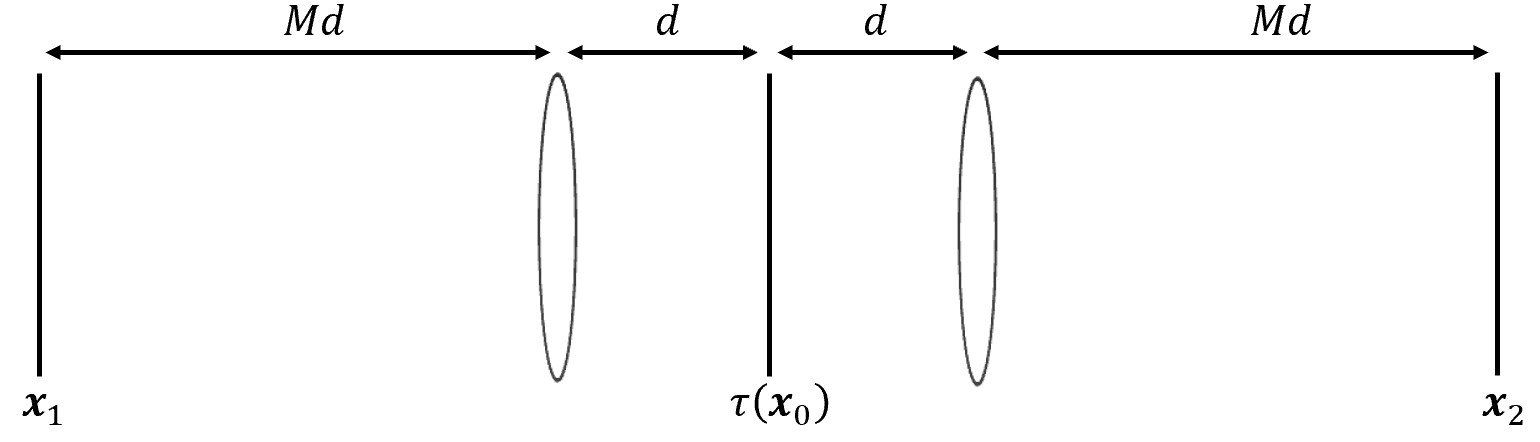
\includegraphics[width=\textwidth]{images/optical_system_schematic.jpg}
	\caption[A simple schematic diagram of a transmissive optical system]{A simple schematic diagram of a transmissive optical system. An aperture mask with amplitude transmittance, $\tau\left(\textbf{x}\right)$, is placed at $\textbf{x}_{0}$. A source with intensity sensitivity described by $S\left(\textbf{x}\right)$ is placed at ${x}_{1}$. A detector with a mask profile described by $D\left(\textbf{x}\right)$ is placed at $\textbf{x}_{2}$. $\textbf{x}_{1}$ and $\textbf{x}_{2}$ are conjugate planes.}
	\label{fig:optical_system_schematic}
\end{figure}

Consider the case of reflection just after the detector mask 
and with the detector aperture positioned at some 
$\textbf{x}_{i}$ such that $S\left(\textbf{x}\right) = 
D\left(\textbf{x}\right) = \delta\left(\textbf{x} - 
\textbf{x}_{i}\right)$, where here $\delta$ denotes the Dirac 
delta function. In this case, assuming an ideal point source, 
the intensity at $\textbf{x}_{i}$ from 
Equation~\ref{eq:intensity_after_detector} becomes:

\begin{equation}\label{eq:confocal_image_form}
I\left(\textbf{x}_{i}\right) = \left| \int h_{1}\left(\textbf{x}\right) h_{2}\left(\textbf{x}\right) \tau\left(\textbf{x} - \frac{\textbf{x}_{i}}{M}\right)d\textbf{x}\right|^{2},
\end{equation}

which is the equation which describes image formation in 
conventional confocal microscopes\cite{wilson1990confocal}.
This describes the image formation from a single point source 
and hence requires scanning in $\textbf{x}_{i}$ to form a 
complete image of the field of view of the object. To remove 
the need for scanning, the source and detector masks should 
instead be composed of an array of pixels with variable 
transmittance where each pixel's transmittance is time 
dependent, $b_{i}\left(t\right)$. The source and detector 
masks can then be described by:

\begin{equation}\label{eq:detector_aperture_time}
S\left(\textbf{x}\right) = D\left(\textbf{x}\right) = \sum_{i=0}^{N} b_{i}\left(t\right)\delta\left(\textbf{x} - \textbf{x}_{i}\right)
\end{equation}

Where $N$ is the number of pixels and each pixel has a 
coordinate $\textbf{x}_{1}, \textbf{x}_{2},...,\textbf{x}_{N}$. 
The resultant image is given by the time average of 
Equation~\ref{eq:intensity_after_detector}:

\begin{equation}\label{eq:confocal_image_time_ave}
\left\langle I\left(\textbf{x}_{2}\right)\right\rangle = \left\langle \int S\left(\textbf{x}_{1}\right) D\left(\textbf{x}_{2}\right) \left| \int h_{1}\left(\textbf{x}_{0} + \frac{\textbf{x}_{1}}{M}\right) \tau\left(\textbf{x}_{0}\right) h_{2}\left(\textbf{x}_{0} + \frac{\textbf{x}_{2}}{M}\right)d\textbf{x}_{0}\right|^{2}d\textbf{x}_{1}\right\rangle,
\end{equation}

where $\left\langle . \right\rangle$ is the time average. 
Since the only time-dependent components are 
$S\left(\textbf{x}_{1}\right)$ and $D\left(\textbf{x}_{2}\right)$ 
only the time average of 
$S\left(\textbf{x}_{1}\right) D\left(\textbf{x}_{2}\right)$ 
need be considered:

\begin{equation}\label{eq:SD_time_ave}
\left\langle S\left(\textbf{x}_{1}\right) D\left(\textbf{x}_{2}\right)\right\rangle = \sum_{i=0}^{N}\sum_{j=0}^{N} \left\langle b_{i}\left(t\right) b_{j}\left(t\right)\right\rangle \delta\left(\textbf{x}_{1} - \textbf{x}_{i}\right) \delta\left(\textbf{x}_{2} - \textbf{x}_{j}\right).
\end{equation}

The transmittance of each pixel should be entirely 
uncorrelated with the transmittance of any other pixel. 
Therefore, a sequence of transmittances is chosen such that:

\begin{equation}\label{eq:pixel_uncorrelation}
\left\langle b_{i}\left(t\right) b_{j}\left(t\right)\right\rangle = \delta_{ij},
\end{equation}

where $\delta_{ij}$ is the Kronecker delta. $b_{i}\left(t\right)$ 
can therefore be any orthonormal sequence, such as an infinite, 
random sequence of $\pm1$ or finite-length complementary Golay 
sequence\cite{golay1949multi}. Unfortunately, such sequences 
require negative transmittance values which is not optically 
achievable. By adding a DC shift this limitation can be overcome 
and the pixel transmissivities become:

\begin{equation}\label{eq:detector_aperture_time_DC}
S\left(\textbf{x}\right) = D\left(\textbf{x}\right) = \frac{1}{2} \sum_{i=0}^{N} \left[b_{i}\left(t\right) + 1\right]\delta\left(\textbf{x} - \textbf{x}_{i}\right).
\end{equation} 

So, the pixel transmissivities, $\frac{1}{2}\left[1 + b_{i}\left(t\right)\right]$, alternate between $0$ and $1$ as $b_{i}\left(t\right)$ 
varies between $\pm1$. Imposing the additional requirement that 
$\left\langle b_{i}\left(t\right) \right\rangle = 0$, then 
Equation~\ref{eq:SD_time_ave} becomes:

\begin{equation}\label{eq:SD_time_ave_DC}
\begin{split}
\left\langle S\left(\textbf{x}_{1}\right) D\left(\textbf{x}_{2}\right)\right\rangle &= \frac{1}{4} \sum_{i=0}^{N}\sum_{j=0}^{N} \left\langle \left[b_{i}\left(t\right) + 1\right] \left[b_{j}\left(t\right) + 1\right] \right\rangle \delta\left(\textbf{x}_{1} - \textbf{x}_{i}\right) \delta\left(\textbf{x}_{2} - \textbf{x}_{j}\right)\\
&= \frac{1}{4} \left[\sum_{i=0}^{N} \delta\left(\textbf{x}_{1} - \textbf{x}_{i}\right) \delta\left(\textbf{x}_{2} - \textbf{x}_{i}\right) + \sum_{i=0}^{N}\sum_{j=0}^{N} \delta\left(\textbf{x}_{1} - \textbf{x}_{i}\right) \delta\left(\textbf{x}_{2} - \textbf{x}_{j}\right)\right].\\
\end{split}
\end{equation}

Substituting Equation~\ref{eq:SD_time_ave_DC} into Equation~\ref{eq:confocal_image_time_ave} 
yields two terms. The first term is the same form as 
Equation~\ref{eq:confocal_image_form} i.e. a conventional 
confocal image. The second term is a non-confocal image 
where all the pixel transmissivities are the same. At the 
limit, where all pixels are adjacent and there is no space 
in between them, then $S\left(\textbf{x}\right) = 
D\left(\textbf{x}\right) = \Sigma_{i=1}^{N}\delta\left(
\textbf{x} - \textbf{x}_{i}\right) = 1$ i.e. a purely 
conventional image\cite{juskaitis1996efficient,wilson1996confocal}. 
Therefore, the image formed by the transmitted light, $I_{T}$, 
is a composite of a conventional and confocal image:

\begin{equation}\label{eq:transmitted_image}
I_{T} = I_{conf} + I_{conv},
\end{equation}

where $I_{conf}$ and $I_{conv}$ are the confocal and 
conventional images respectively. Instead of an array of 
pixels with programmable transmissivity, the Aurox Clarity 
module implements a disk with a photolithographed 
transmittance sequence. In this case, the transmittance 
pattern presented to a given fixed pixel is equivalent to 
the transmittance pattern along the corresponding arc of 
the disk\cite{wilson1996confocal}. 
Equation~\ref{eq:detector_aperture_time_DC} should therefore 
be modified to:

\begin{equation}\label{eq:detector_aperture_arc}
S\left(\textbf{x}\right) = D\left(\textbf{x}\right) = \frac{1}{2} \sum_{i=0}^{N} \left[b_{i}\left(\textbf{x}_{r}\right) + 1\right]\delta\left(\textbf{x} - \textbf{x}_{i}\right),
\end{equation}

where $\textbf{x}_{r}$ is the rotation coordinate. In 
this case, the final image is obtained by averaging over 
$\textbf{x}_{r}$ rather than over time, but the result is 
still Equation~\ref{eq:transmitted_image}. Previous 
implementations of this approach acquired two images, the 
second of which had $b_{i}\left(\textbf{x}_{r}\right) = 1$ 
i.e. no aperture mask. As Figure~\ref{fig:aurox_clarity_internal} 
shows, the Aurox clarity module images both the light 
transmitted through the spinning disk and the light 
reflected off the disk where the transmissivity is $0$. In 
this case, the detector mask is defined as:

\begin{equation}\label{eq:detector_aperture_arc_reflect}
D\left(\textbf{x}\right) = \frac{1}{2} \sum_{i=0}^{N} \left[1 - b_{i}\left(\textbf{x}_{r}\right)\right]\delta\left(\textbf{x} - \textbf{x}_{i}\right).
\end{equation}

Applying the same average over $\textbf{x}_{r}$ as before, 
the image formed by the reflected light, $I_{R}$, is:

\begin{equation}\label{eq:reflected_image}
I_{R} = I_{conv} - I_{conf}.
\end{equation}

Therefore, both the confocal and conventional images can 
be recovered by:

\begin{equation}\label{eq:confocal_image}
I_{conf} = \frac{1}{2}\left(I_{T} - I_{R}\right),
\end{equation}

\begin{equation}\label{eq:conventional_image}
I_{conv} = \frac{1}{2}\left(I_{T} + I_{R}\right).
\end{equation}

This has the benefits of only requiring one exposure for 
the sample to acquire a confocal image and using all of 
the emitted fluorescence light. The spinning disk in the 
Clarity module has three different grid patterns with 
different spacing. The spacing of the grid pattern determines
the degree of optical sectioning and so these grid patterns
represent low, medium and high optical sectioning\cite{neil1997method}. Low sectioning uses the coarsest disk pattern and leads to a thicker optical section (2.5 $\mu$m, as specified by the manufacturer); the medium spaced pattern has a slightly smaller section (1.7 $\mu$m); the finest spacing corresponds to a thinner optical section (0.9 $\mu$m)\cite{hussain2020wavefront}. 

\section{DeepSIM}
\label{sec:DeepSIM}

As discussed in Section~\ref{subsec:SIM}, 3D structured illumination microscopy (3D-SIM) is a super-resolution 
microscopy technique which is well suited to imaging live biological samples 
due to the relatively few images required to reconstruct a super-resolution 
image, millisecond temporal resolution, medium energy load, true multi-colour 
imaging and fast volume 
acquisition\cite{schermelleh2010guide,schermelleh2019super,schermelleh2008subdiffraction}.
However, to date this application has not been extensively exploited for all 
live sample preparations, namely those requiring dissection and bathing, and 
those requiring dynamic sample manipulation such as electrophysiology 
experiments. This is for two principle reasons. Firstly, these biological 
samples have to be suspended in usually aqueous  media to sustain them, which 
necessitates an upright configuration. To date, no upright 3D-SIM system 
exists since this configuration is more challenging to achieve and it is 
only required for specific biological applications. The aqueous nature of 
the suspension media also precludes the use of 
oil objectives, reducing the available NA and hence resolution. Secondly, 
imaging at depths $>20\mu m$ remains a challenge for traditional 3D-SIM 
methods due to limited background rejection and optical aberrations degrading 
the stripe contrast necessary for successful SIM imaging\cite{wu2018faster}. 
Aberrations pose a larger issue in live sample imaging compared to fixed 
sample imaging, not least of all because live samples cannot be cleared of 
the extraneous biological structures. Therefore, most 3D-SIM imaging has been 
limited to thin specimens\cite{weil2010distinguishing}. DeepSIM is a bespoke 
microscope designed to address these issues. It is an open and flexible 
upright microscope platform to enable imaging in live samples requiring 
dynamic manipulation. Incorporating a spatial light
modulator (SLM) to generate the structured 
illumination pattern enables rapid 3D, multi-colour SIM data acquisition. 
Finally, incorporating adaptive optics allows for SIM imaging at 
unprecedented depths in live samples, as well as remote focusing which 
further increases the speed of image acquisition whilst minimising motion 
artifacts. The DeepSIM optical design inherits elements and insights from 
both the OMX system\cite{haase2008omx,dobbie2011omx} and, later, the 
CryoSIM system\cite{phillips2020cryosim}.

\subsection{DeepSIM Optical Set-up}
\label{subsec:DeepSIM_optics}

Figure~\ref{fig:DeepSIM_complete_beam_paths} shows the complete
optical schematic of the DeepSIM microscope. There are multiple
possible beam paths which can be altered by raising/lowering certain
optics and/or pairs of mirrors. The solid green path denotes the
primary 3D-SIM excitation path. The laser beams are combined at a
single exit port, magnified and then reflected onto SLM at a shallow 
angle ($<10^{\circ}$). The SLM acts as a programable phase grating 
imposing the structure to the illumination pattern required for SIM 
imaging. The beam is then magnified and reimaged onto the Alpao 
69-actuator DM. The SLM and DM are in reciprocal planes to one another. 
The SLM is placed in a plane conjugate to the imaging plane in order to 
create the structured illumination pattern as the imaging plane. The DM 
is placed in a plane conjugate to the pupil plane since, as discussed in 
Section~\ref{sec:aberrations}, the aberrations present are described by a 
pupil function. The beam is then demagnified and imaged on the LUMFLN60XW 
$60\times$ water dipping objective. The emission beam path follows the 
same path in reverse up until past the DM. At this point the emission 
beam path is redirected by a dichroic mirror (Chroma Technology 
ZT405/488/561/640rpc), magnified and then reimaged onto the Andor iXon 
Ultra EMCCD cameras. There is a secondary dichroic (Chroma Technology 
ZT561rdc-xr) which separates the ``red'' colour channel (562nm-800nm) 
from the ``green'' colour channel (390nm-562nm). Since the DM is in both 
the excitation and emission paths it is able to correct for aberrations 
in both paths.

\begin{figure*}
	\centering
	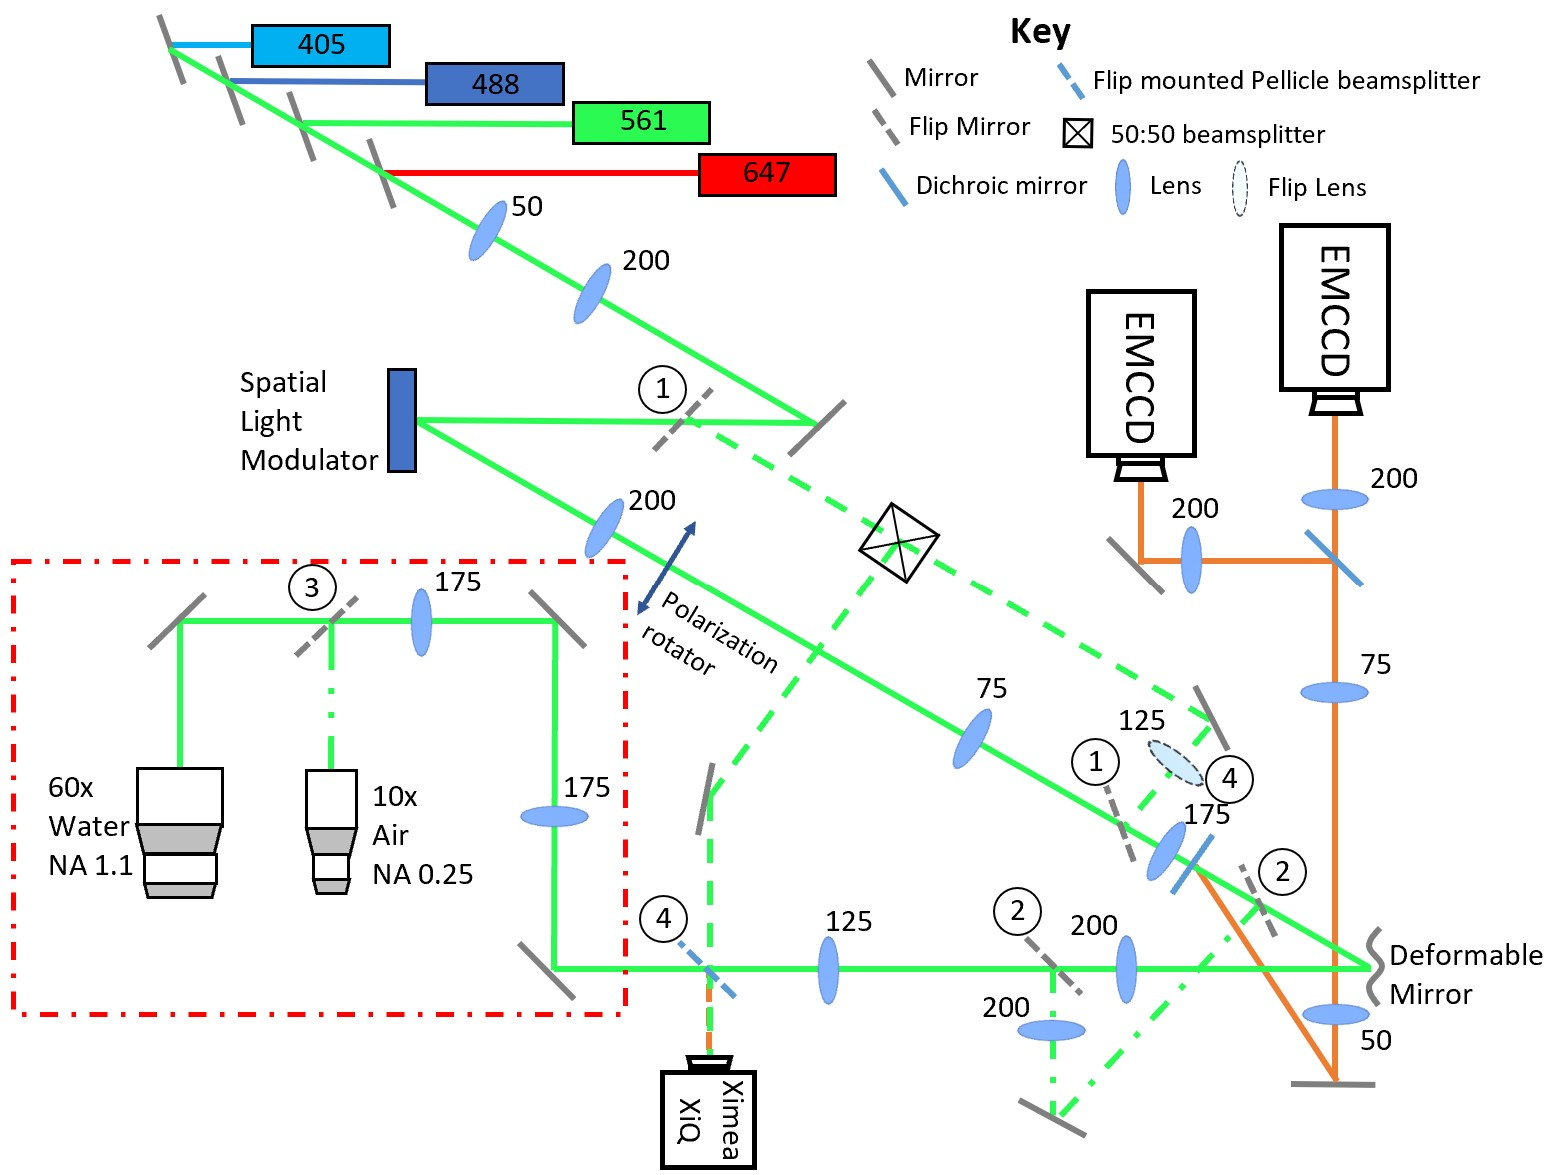
\includegraphics[width=\textwidth]{images/DeepSIM_complete_beam_paths_upright.jpg}
	\caption[Complete beam path layout for DeepSIM.]{Complete beam path layout for DeepSIM. DeepSIM has multiple paths that can be selected by flipping the numbered pairs/individual mirrors. The green paths denotes the excitation beam paths. The solid green path shows the structured illumination (SI) beam path. The dashed green path shows the widefield beam path. This is changed to the interference beam path by flipping up the lens and pellicle pair. The dot-dashed green path shows the excitation path which bypasses the deformable mirror. The dot-dot-dashed green path shows the excitation path going through the $10\times$ air objective for low magnification sample mapping. The orange path denotes the emission beam path. The area denoted by the red dot-dash outline is mounted perpendicular to the optical table.}
	\label{fig:DeepSIM_complete_beam_paths}
\end{figure*}

Raising the \circled{1} pair of flip mirrors bypasses the SLM and changes the excitation beam path to a widefield configuration. Raising the \circled{2} pair of flip mirrors bypasses the DM. This is a useful configuration when the DM has not yet been calibrated since the neutral position of the DM actuators have a worse flatness profile than that of a plane mirror. Without calibration, the DM surface cannot be flattened and may contribute to the aberrations present in the imaging system. Raising the \circled{3} flip mirror directs the excitation beam path through the $10 \times$ air objective. This beam path is used for large field of view (FOV) mapping.

Raising both the \circled{1} pair of flip mirrors and the \circled{4}
flip mounted pellicle beamsplitter and lens changes both the
excitation and emission beam paths to create an interferometer. Half
of the excitation beam is picked off by the 50:50 beamsplitter and
directed straight into the Ximea XiQ camera. This is the
interferometer reference arm. The sample beam arm proceeds through the
regular excitation beam path. Placing a mirror in the focal plane of
the $60\times$ objective reflects the beam back through the emission
beam path until it is reflected by the pellicle into the Ximea XiQ
camera. The interference pattern produce by the two beams can be interrogated to yield an image of the wavefront phase. Since the DM is in the sample arm, varying the shape of the DM surface will change the shape of the phase wavefront. Measuring how the movement of the DM's actuators influences the shape of the phase wavefront allows the DM to be calibrated and subsequently used to correct for aberrations in the optical system or sample. 

\subsection{Optical Alignment}
\label{subsec:alignment}

Being a bespoke microscopy system, DeepSIM was assembled from individual components and aligned by hand. This alignment process is critical for ensuring the microscopy system itself introduces the smallest possible aberrations. Aberrations in the imaging system disrupt image formation and degrade image quality\cite{wyant1992basic}. This affects both the excitation and emission paths of any fluorescent microscope. For a SIM microscope such as DeepSIM the most noticeable effect in the excitation path is the degradation of the structured illumination pattern, particularly the high spatial frequency components\cite{debarre2008adaptive,booth2015aberrations}. In the emission path, these aberrations prevent correct image formation on the camera's sensors. Whilst DeepSIM incorporates a DM for performing aberration correction, every DM has a limited stroke and the actuator response is often non-linear at the limits of this stroke. Correcting for relatively large system aberrations due to a poorly aligned system is likely to lead to insufficient remaining stroke to correct for sample induced aberrations. Therefore, having a well aligned system is still critical even for AO-enabled microscopy systems such as DeepSIM.

Firstly, the upright bridge to hold the objectives and the stage in their upright configuration was constructed and installed on the optical table. One of the lasers was then installed and the beam paths shown in Figure~\ref{fig:DeepSIM_complete_beam_paths} was constructed without the lenses. The beam was kept either parallel or perpendicular to the optical table where appropriate and passing through the centre of the objective aperture. The beam was kept parallel to the table by positioning an iris at the beam height of the laser and 'walking' this iris down the beam path, ensuring that after each reflection the beam remains at the same height. Once this beam path was established, the lenses were added sequentially and aligned. Finally, the other lasers were coaligned to this beam path. The result is the complete optical setup shown in Figure~\ref{fig:DeepSIM_physical_optics}.

\begin{figure}[h]
	\centering
	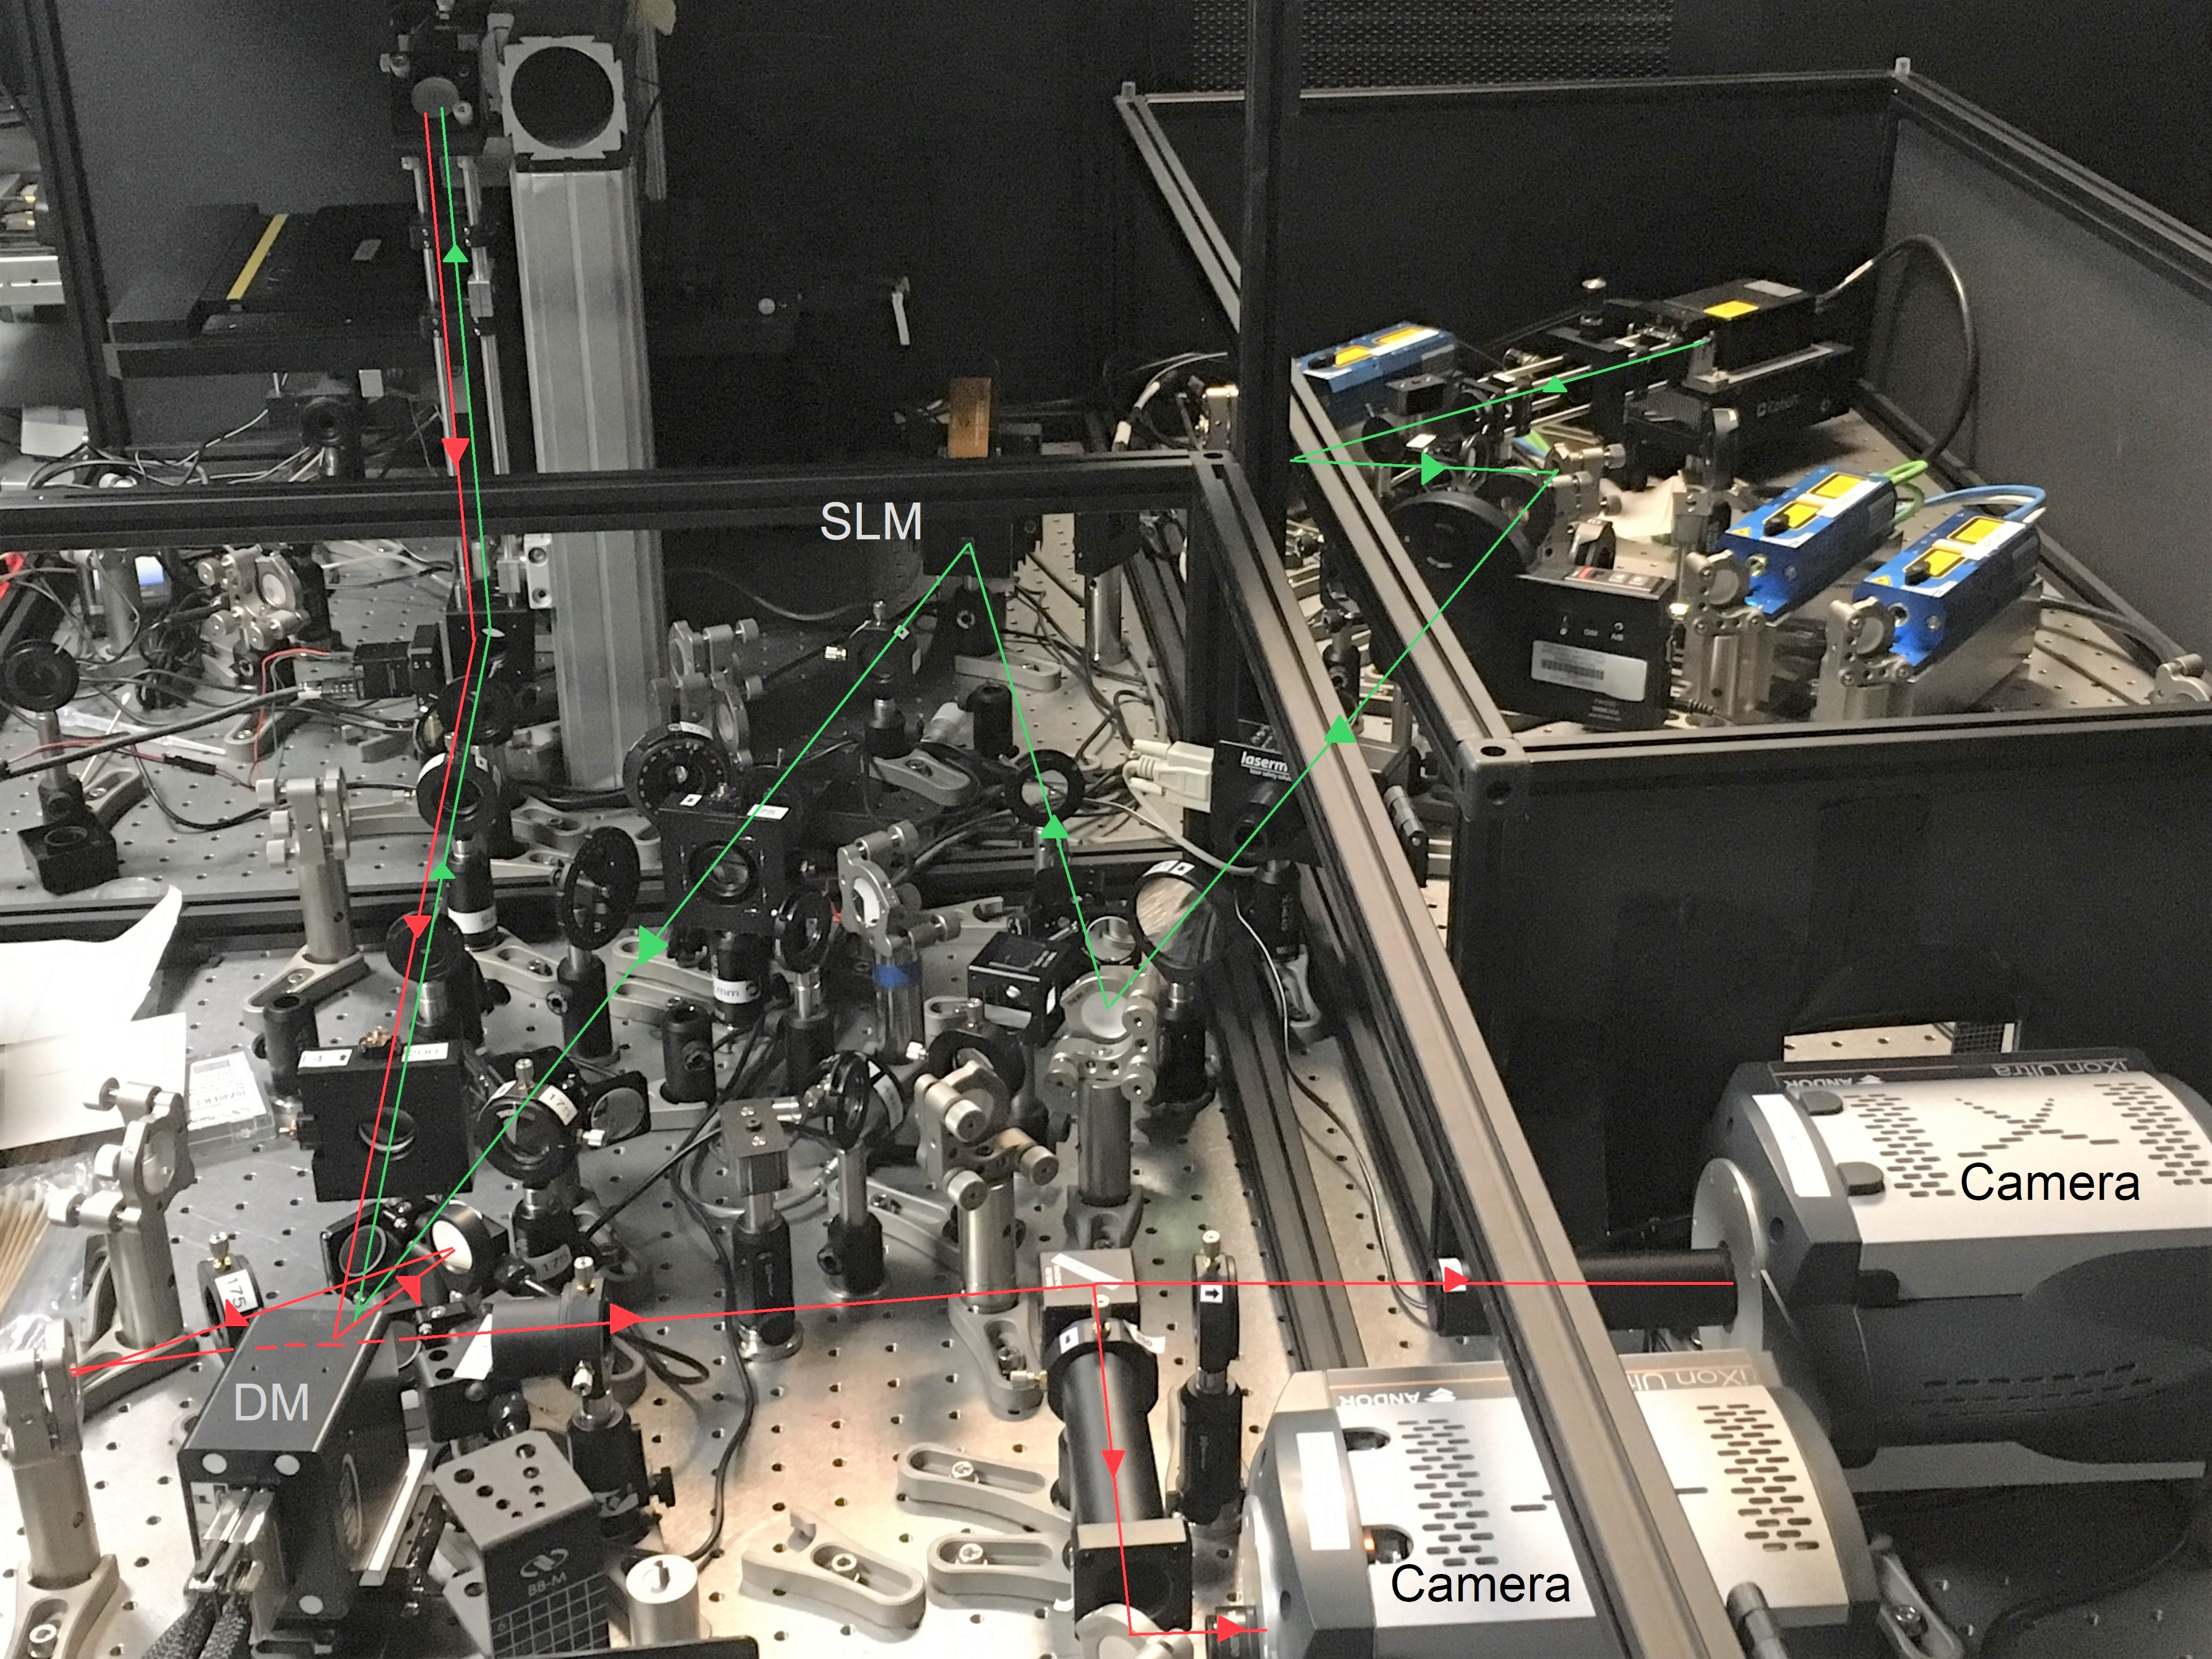
\includegraphics[width=\textwidth]{images/DeepSIM_SIM_path_annotated_bright.jpg}
	\caption[The aligned DeepSIM optical set-up.]{The aligned DeepSIM optical set-up. The 3D-SIM excitation (green) and emission (red) beam paths are annotated.}
	\label{fig:DeepSIM_physical_optics}
\end{figure}

The alignment of the lenses and the coalignment of the lasers is typically done by eye.  Typically,
systems are initially aligned with a small beam and no lenses.
Pinholes or irises are placed at critical points in
the optical system and then a light beam, usually a laser with
a low divergence angle, is aligned to these points. Lenses
are then added one at a time. Once a lens is added,
propagation of the beam is checked further along the optical
path to ensure the beam is passing through the centre of the
lens and the lens angle is judged by ensuring the back
reflections are centred on the incident beam. This process is
repeated for each lens. The quality of the alignment
depends upon significant expertise and subjective judgement to
both see how well aligned the beam is and to decide when it is
sufficiently well aligned to move on to the next element in
the system.

This approach has two obvious problems. The first is that the
human eye has limited resolving power of approximately 3 to 6
arcseconds \cite{ogle1951resolving}. At a distance of 50$\mu$m,
this is a resolution limit of approximately 10$\mu$m. This doesn't account for parallax errors which
can further reduce the resolution and introduce systematic
errors, nor does is account for the user's ability to
accurately judge the comparison between where a laser spot
currently is and where it was at some point in the past
\cite{mardanbegi2012parallax}. The second problem is that this
method of alignment requires users to stare at diffuse laser
reflections for extended periods of time which carries an
inherent safety risk \cite{sliney1995laser}. Again, this
problem can be exacerbated if a user tries to minimise the
parallax errors and get level with the optical axis as they
then run the risk of accidentally observing collimated laser
light or specular reflections. 

Errors introduced during alignment contribute optical aberrations even before any heterogeneous sample is imaged. This leads to lower quality imaging in systems without adaptive elements. For systems such as DeepSIM with adaptive elements, these aberrations can be corrected for by the adaptive elements. However, since adaptive elements such as deformable mirrors have a finite stroke length, utilising a portion of these elements corrective capacities correcting for the system aberrations present means less corrective power can be levelled against the aberrations caused by the samples of interest. This is a needless expenditure of corrective power when these system aberrations can be minimised by  improving the alignment quality by other means.

BeamDelta is an optical alignment tool designed to address both of the problems with the traditional approach to optical alignment. The laser is imaged directly on two cameras at different positions and the beam centroid positions are calculated for each camera image. These centroid positions can be stored and then subsequent centroid positions - such as those of other lasers which are being coaligned or the original beam after the addition of a lens - can be measured relative to these reference positions. This allows for optical alignment which is several orders of magnitude more accurate and considerably safer than the traditional method of aligning components by eye\cite{dobbie2019beamdelta}. It also has the benefit of making the whole process considerably more efficient. DeepSIM required multiple realignments which prior to the development of BeamDelta would take at least a week. With BeamDelta, a complete realignment of the system took only a couple of days.

\section{Control Software}
\label{sec:control_software}

\subsection{\textit{Python Microscope}}
\label{subsec:microscope}

There is a requirement for control over all the hardware elements of
an optical system. This can pose a problem since each hardware
component has its own low-level software libraries and the physical
hardware is connected to several different computers. Additionally, in
order to ensure rapid imaging of 3D widefield and SIM Z-data stacks
there is a requirement for precise timing control of the electronic
hardware, such as laser, cameras, etc, which must act in concert. To
solve these challenges, hardware on both the Aurox Clarity and DeepSIM
systems are controlled via Python Microscope, an open source Python
package which allows the various elements to be synchronised with
hardware triggers.\cite{pinto2021python} For this, a RedPitaya, a commodity single board
computer, is used on each system and
functions as a dedicated hardware timing controller.

\subsection{\textit{Microscope-Cockpit}}
\label{subsec:cockpit}

Modern complex optical systems require a bespoke graphical user interface (GUI) which is accessible to users. For this purpose, Microscope-Cockpit, a highly flexible and adaptable open source Python-base GUI environment, is utilised for both systems.\cite{phillips2021microscope} Figure~\ref{fig:Cockpit_UI} shows the GUI used to control both systems. In the main window, Figure~\ref{fig:DeepSIM_control_software_main_window}, a user can enable and disable the various hardware elements. They can also swap between the various beam paths shown in Figure~\ref{fig:DeepSIM_complete_beam_paths}. A user also has access to the automated AO methods, the specifics of which will be discussed later. Figure~\ref{fig:DeepSIM_control_software_stage_control} shows the window which can be used to control the XY stage, and the coarse mechanical and fine piezo Z stages as well as display the location of each. The step control and step size for each of these are assigned to keyboard shortcuts. 

\begin{figure}[h]
	\centering
	\begin{subfigure}[t]{0.575\textwidth}
		\centering
		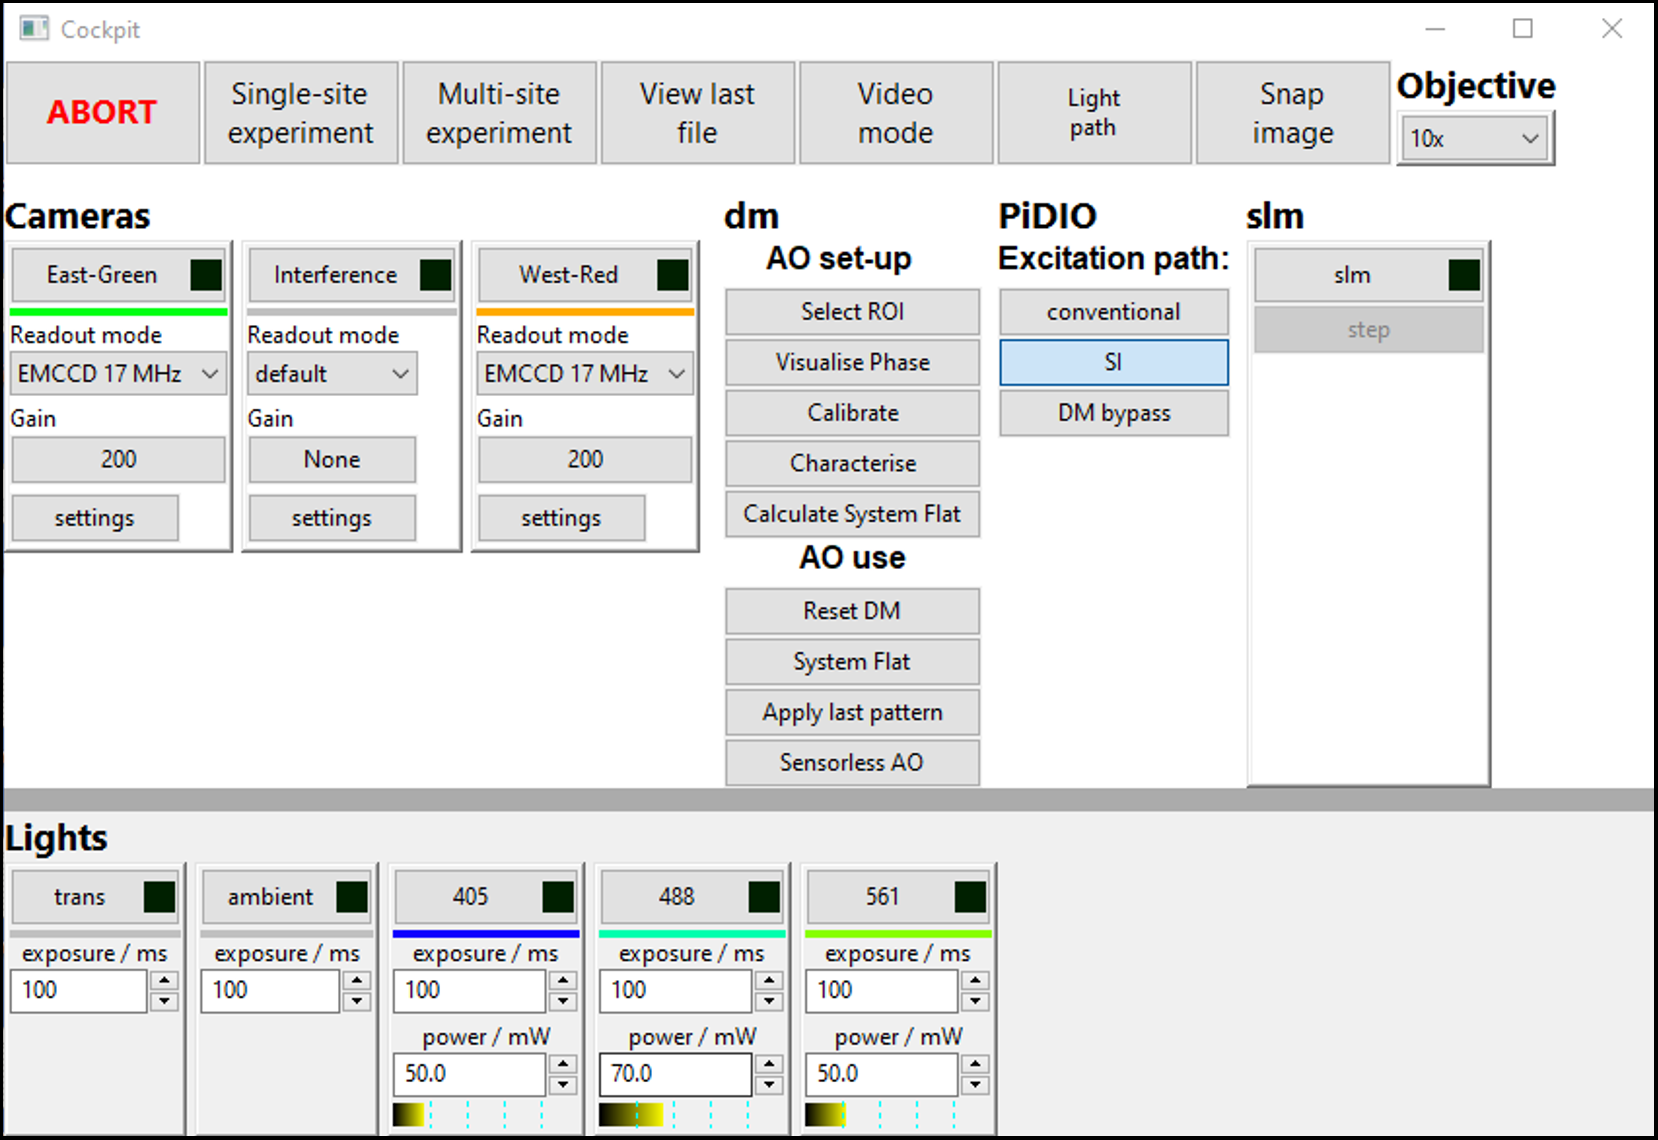
\includegraphics[width=\linewidth]{images/cockpit_GUI_main.png}
		\caption{}
		\label{fig:DeepSIM_control_software_main_window}
	\end{subfigure}
	\begin{subfigure}[t]{0.3325\textwidth}
		\centering
		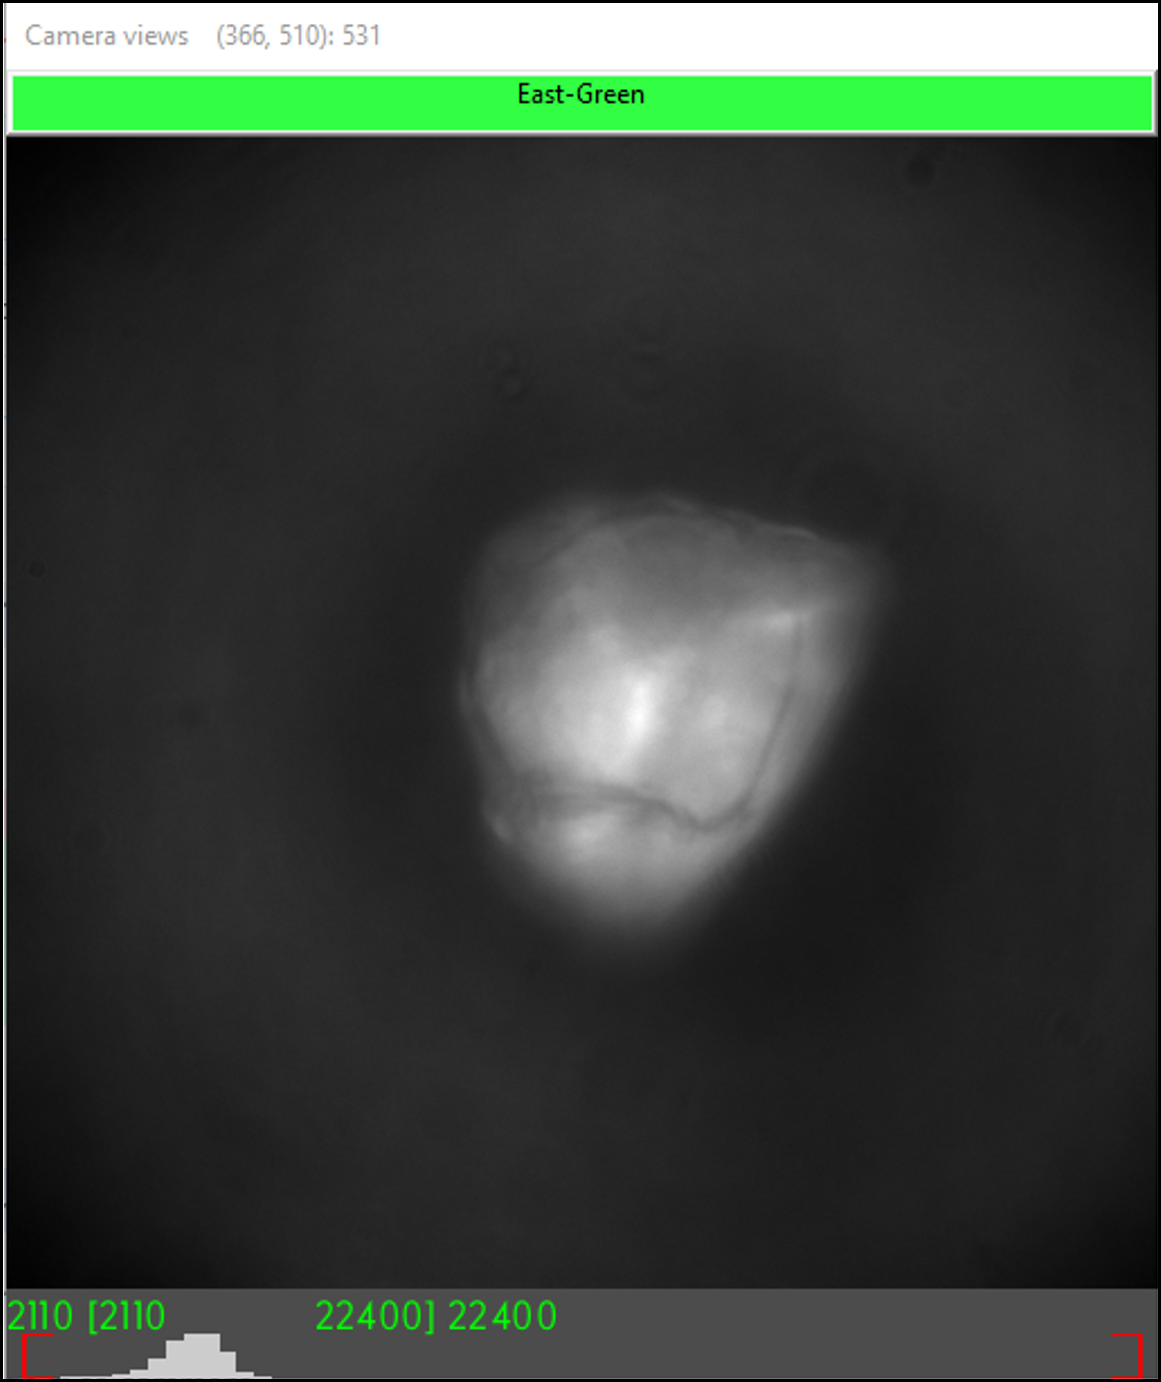
\includegraphics[width=\linewidth]{images/cockpit_GUI_camera.png}
		\caption{}
		\label{fig:DeepSIM_control_software_camera}
	\end{subfigure}
	
	\begin{subfigure}[t]{0.51\textwidth}
		\centering
		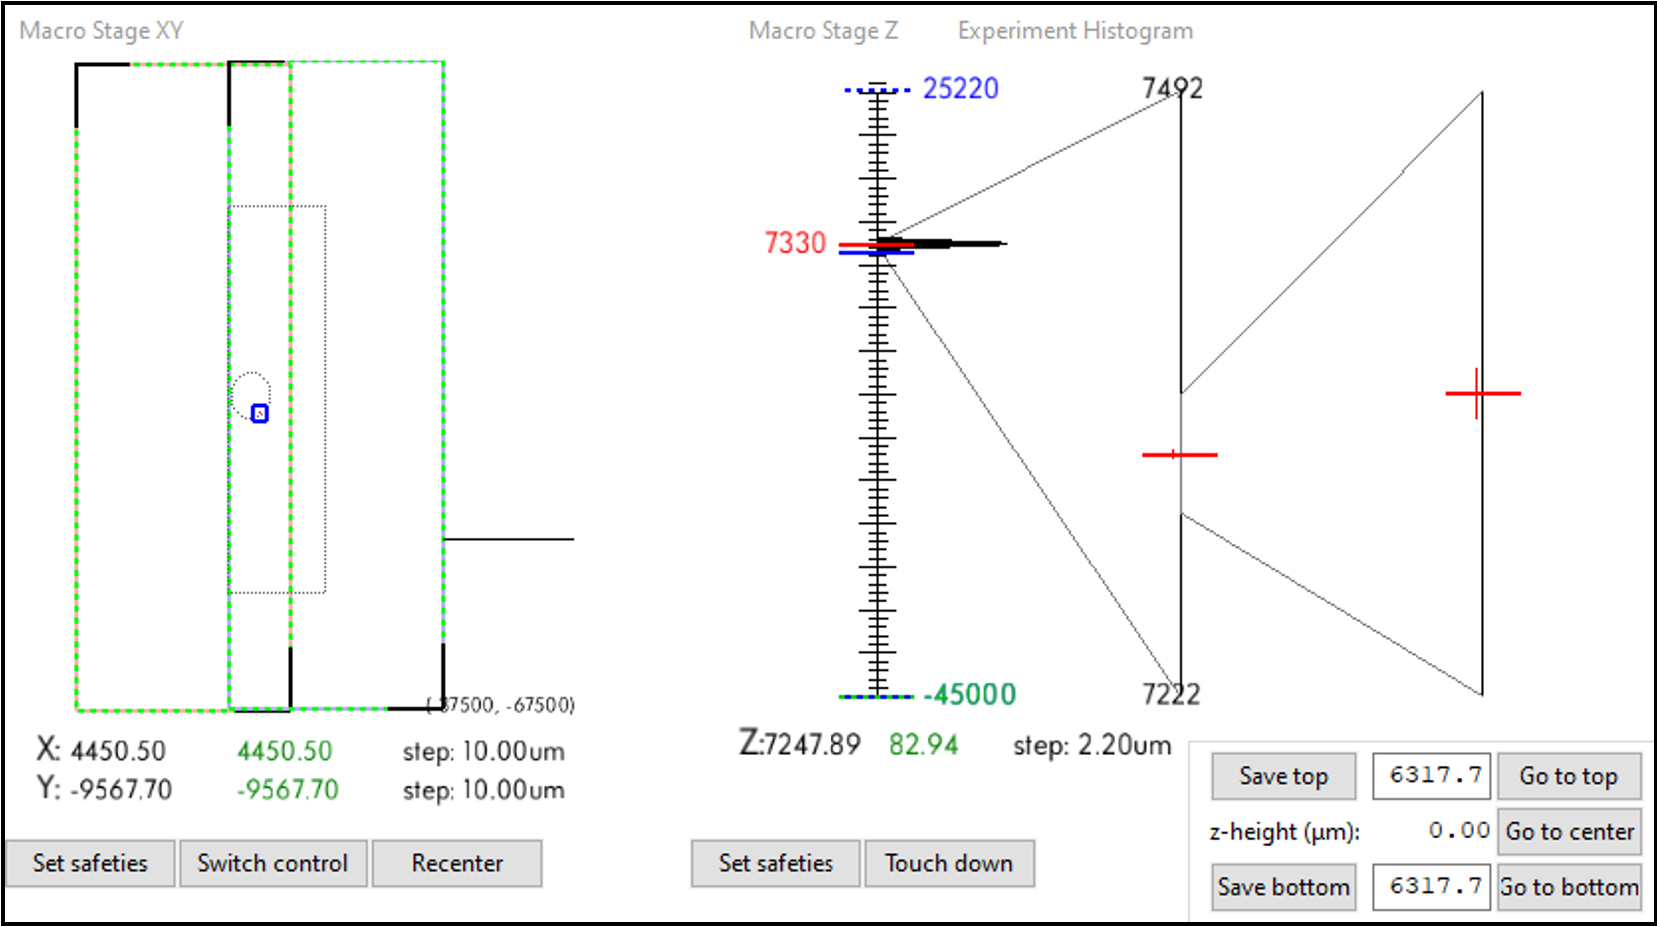
\includegraphics[width=\linewidth]{images/cockpit_GUI_stage.png}
		\caption{}
		\label{fig:DeepSIM_control_software_stage_control}
	\end{subfigure}
	\begin{subfigure}[t]{0.445\textwidth}
		\centering
		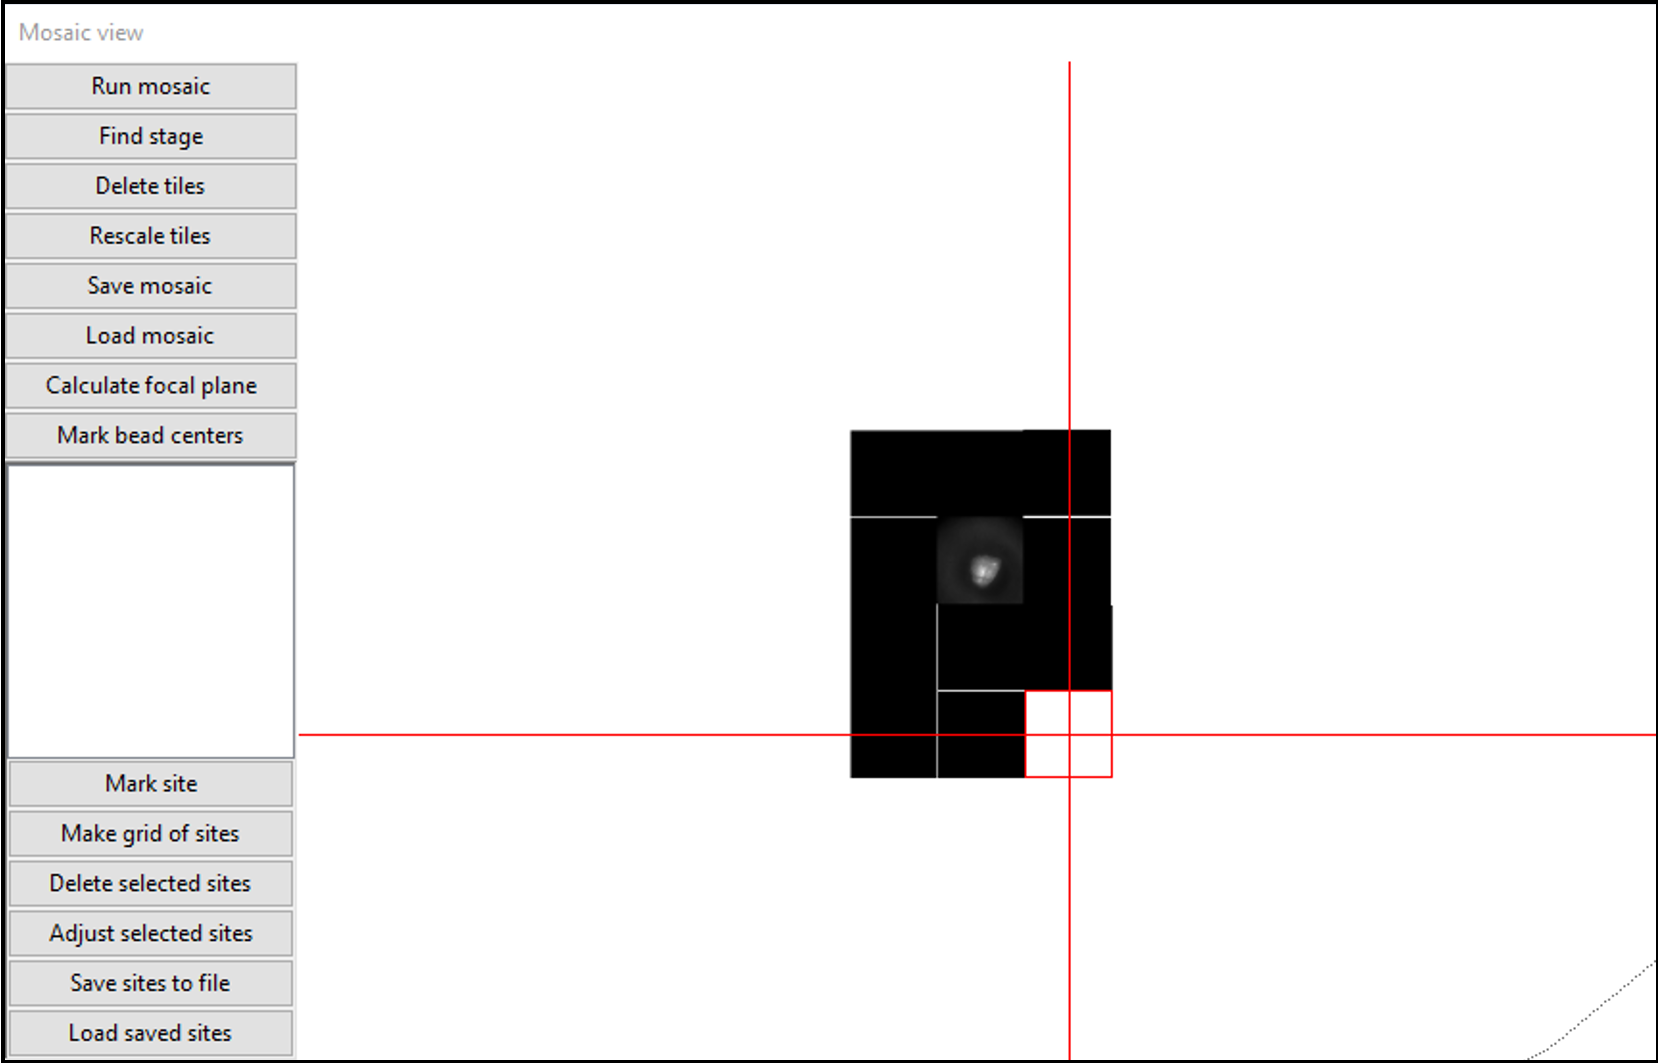
\includegraphics[width=\linewidth]{images/cockpit_GUI_mosaic.png}
		\caption{}
		\label{fig:DeepSIM_control_software_mosaic}
	\end{subfigure}
	\caption[Microscope-Cockpit GUI for controlling DeepSIM]{Microscope-Cockpit GUI for controlling DeepSIM \textbf{(a)} Microscope-Cockpit main window. Contains buttons to enable all the hardware, set laser powers and change beam paths \textbf{(b)} Camera view window. Shows the most recent readout from all the enabled cameras \textbf{(c)} Stage control window. Allows the user to control the position of the XY piezo-stage, coarse mechanical Z stage and fine Z piezo-stage \textbf{(d)} Mosaic window. Used by the user to scan the field of view for structures of interest and mark them.}
	\label{fig:Cockpit_UI}
\end{figure}

Unlike most commercial microscopes, DeepSIM does not have any eyepieces. Ordinarily this would present a problem for simply locating the sample, let alone locating a specific region or structure of interest within the sample. To overcome this limitation, Microscope-Cockpit implements a Mosaic window shown in Figure~\ref{fig:DeepSIM_control_software_mosaic}. When the mosaic is run, Microscope-Cockpit moves the stage in an anti-clockwise spiral pattern and takes a widefield image at each position. These images are stored on the main machine's graphics card to enable real-time navigation and site-of-interest marking. Since the images are stored, a user can revisit and investigate areas of the sample which have already been imaged without re-imaging them, decreasing the light exposure and limiting photodamage. The user is able to take an initial mosaic using the $10\times$ objective to find the sample, create a specimen guide map and identify regions of interest. They then swap to the $60\times$ objective and laterally shift the stage to the location of the previous field of view for a more detailed mosaic in the previously identified regions, locate specific sites of interest which they can then mark. The marked sites can then be visited by the user individually and have data collected manually using the ``Single-site experiment'' option or each site can be visited and data collected in an automated fashion using the ``Multi-site experiment'' option. In this way DeepSIM can function well without eyepieces and is easily controlled by a potential user.

Although the bulk of the Microscope-Cockpit UI was developed by others, the integration of the adaptive optics functionality for both set-up and use was entirely novel. It was designed to be robust and easy to operate by non-specialist users, primarily the biologists using DeepSIM. A complete exploration of the available functionality appears in Chapter~\ref{chpt:ao_tools}.
